\section{Exercise 5.2 Complementary Slackness}
\textbf{Problem:} 

\textbf{Solution:} The goal of the solution is to construct an example in which the standard-form problem (P) has an optimal solution $\hat{x}$ and there exists $\hat{y}$ that is not feasible in its dual dual (D) and is complementary to $\hat{x}$. In this example, there exists multiple $\hat{y}$ that are complementary to $\hat{x}$, yet not all of them are feasible. 

If $b=\mathbf{0}$, then $\hat{x}_\beta = A_\beta^{-1}b = \mathbf{0}$. In this case, it's very easy to find a $\hat{y}$ that is complementary to $\hat{x}$ and the $\hat{y}$ is not a feasible solution of (D). However, we'd like to explore a general case where $b\neq\mathbf{0}$.

Let's first take a look at the definition of \textbf{complementarity}.

\newtheorem{mydef}{\emph{\textbf{Definition}}}
\begin{mydef}
With respect to the standard-form problem (P) and its dual (D), the solutions $\hat{x}$ and $\hat{y}$ are \textbf{complementary} if 

\[
\begin{array}{rccl}
 (c_j-\hat{y}'A_{\cdot j})\hat{x}_j &  = & 0~,& \text{for}~j=1,2,...,n ~; \\
 \hat{y}_i(A_{i\cdot}\hat{x}-b_i) & = & 0~, & \text{for}~i=1,2,...,m ~.
\end{array}
\]

\end{mydef}

Given that $\hat{x}$ is optimal, $\hat{x}$ is the basic feasible solution of (P). So

\[
\begin{array}{rcl}
 A\hat{x} &=& b~, \\
 \hat{x} &\geq& \mathbf{0}~.
\end{array}
\]

which means $A_{i\cdot}\hat{x}-b_i = 0,\text{for}~i=1,2,...,m$, so the second equation for complementarity is satisfied: $\hat{y}_i(A_{i\cdot}\hat{x}-b_i) = 0$. Since $\hat{x}$ is a basic solution, $\hat{x}_{\eta} = 0$, so $(c_{\eta_j}-\hat{y}'A_{\cdot \eta_j})\hat{x}_{\eta_j} = 0~, \text{for}~j=1,2,...,n-m$. In order to solve $\hat{y}$ given $\hat{x}$, we need to solve the following equations

$$(c_{\beta_j}-\hat{y}'A_{\cdot \beta_j})\hat{x}_{\beta_j} = 0~, \text{for}~j=1,2,...,m~.$$

Given that $\hat{y}$ is m by 1, if none of the $\hat{x}_{\beta_j}, \text{for}~j=1,2,...,m$ is zero, there is unique $\hat{y}$ complementary to $\hat{x}$, which is also the feasible solution of (D). However, if there exists $\hat{x}_{\beta_j}$ that equals zero, there are more than one $\hat{y}$ that complementary to $\hat{x}$, and it is possible to construct one of the $\hat{y}$ to be not feasible of (D) as we can add one more constraint of $c_{\beta_j}-\hat{y}'A_{\cdot \beta_j} < 0$ so that $\hat{y}'A_{\cdot \beta_j} > c_{\beta_j}$ for $\beta_j$ that $\hat{x}_{\beta_j} = 0$. In this way, $\hat{y}'A \leq c'$ does not hold and $\hat{y}$ is not a feasible solution of (D).

To construct an problem (P) with optimal solution $\hat{x}$ such that $\hat{x}_{\beta_j} = 0$ for some $j$, we leverage the geometric explanation of basic and nonbasic variables. Suppose $(\beta, \eta)$ is the partition for the optimal solution, then on the space of nonbasic variables, for the projection of the lines $\left(A_\beta^{-1}A_\eta\right)x_\eta = A_\beta^{-1}b$, there exists one line that is across the origin $(0,0)$. The algebraic explanation of this is that there exists $\hat{x}_{\beta_j} = 0$ for the basic variable.

We leverage this observation to construct the example. We first construct an standard-form problem (P) with $m=3$ and $n=5$ and found the optimal solution through {\tt AMPL}:

\[
\begin{array}{ccc}
\tilde{A}  :=  \left(
  \begin{array}{ccccc}
    1 & -1 & 0 & -1 & 0  \\
    0 & -4 & 2 & 2 & 0 \\
    0 & -9 & 0 & 6 & 3\\
  \end{array}
\right)~, &
\tilde{b}  :=  (1,2,18)'~,&
\tilde{c}  :=  (16, 7, 20, 10, 4)'~.\\

\end{array}
\]

The optimal solution $\hat{\tilde{x}} = (2,0,0,1,4)'$ and the associated partition is $\tilde{\beta} = \{1,4,5\}, \tilde{\eta}= \{2,3\}$. We show the projection onto the space of nonbasic variables in Figure \ref{fig:p11}. We can know that 

\[
\begin{array}{ccc}
\tilde{A}_\beta^{-1}  =  \left(
  \begin{array}{ccc}
    1 & 1/2 & 0   \\
    0 & 1/2 & 0 \\
    0 & -1 & 1/3\\
  \end{array}
\right)~, &

\tilde{A}_\beta^{-1}\tilde{A}_\eta  =  \left(
  \begin{array}{cc}
    -3 & 1   \\
    -2 & 1 \\
    1 & -2\\
  \end{array}
\right)~,&

\tilde{A}_\beta^{-1}\tilde{b}  =  \left(
  \begin{array}{c}
    2   \\
    1 \\
    4\\
  \end{array}
\right)~,

\end{array}
\]

\begin{figure}[h!!]
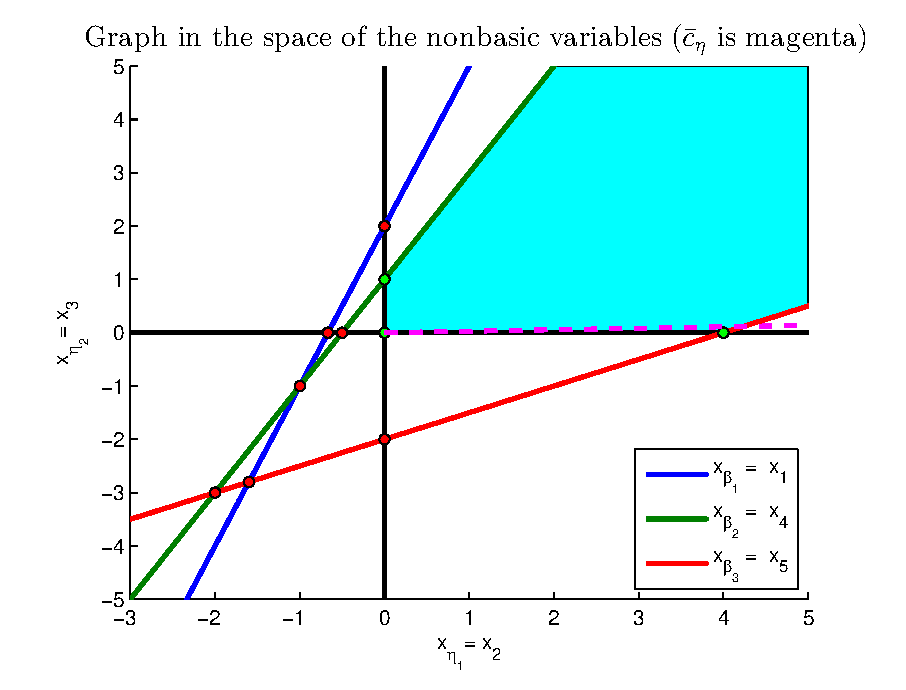
\includegraphics[width=0.7\textwidth]{p2/initial.eps}
\caption{Feasible region projected into the space of $(x_2,x_3)$ with $\tilde{A},\tilde{c},\tilde{b}$}\label{fig:p11}
\end{figure}

Then we add one more basic variable ($x_6$), and corresponding add one more line in the space of nonbasic variables. This line should not affect the feasible region and should be across the origin. We also need to guarantee that other lines are not affected and the optimal solution is kept regarding the original variables. We achieve this by changing the following matrix (the geometric explanation is shown in Figure \ref{fig:p12}):

\[
\begin{array}{ccc}
A_\beta^{-1}  =  \left(
  \begin{array}{cccc}
    1 & 1/2 & 0 & 0  \\
    0 & 1/2 & 0 & 0\\
    0 & -1 & 1/3 & 0\\
    0 & 0 & 0 & 1\\
  \end{array}
\right)~, &

A_\beta^{-1}A_\eta  =  \left(
  \begin{array}{cc}
    -3 & 1   \\
    -2 & 1 \\
    1 & -2\\
    -1 & -1 \\
  \end{array}
\right)~,&

A_\beta^{-1}b  =  \left(
  \begin{array}{c}
    2   \\
    1 \\
    4\\
    0\\
  \end{array}
\right)~,

\end{array}
\]

\begin{figure}[h!!]
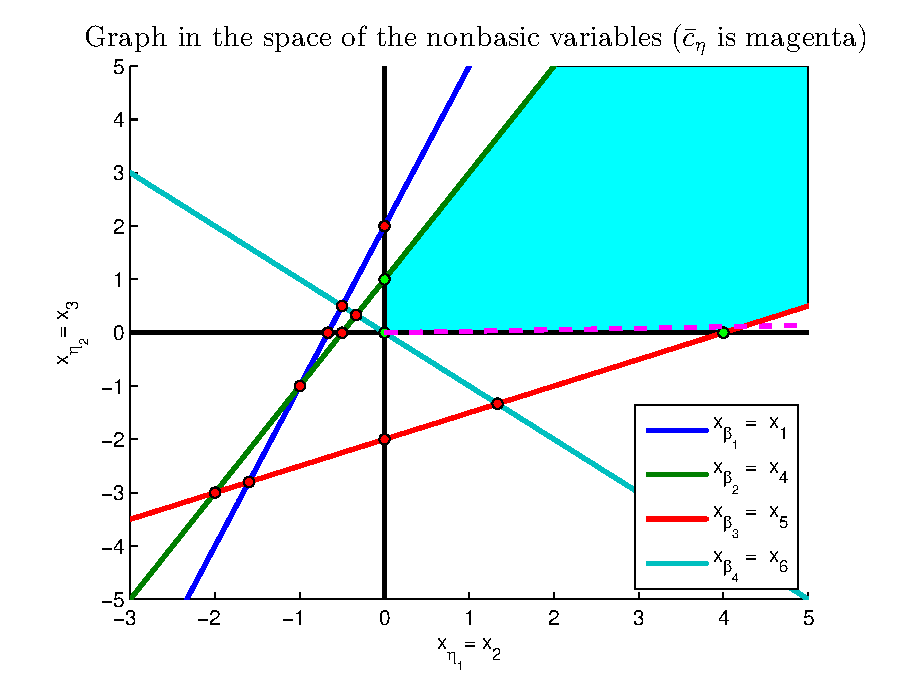
\includegraphics[width=0.7\textwidth]{p2/new.eps}
\caption{Feasible region projected into the space of $(x_2,x_3)$ with $A,c,b$}\label{fig:p12}
\end{figure}

We then solve $A_\eta$ and $b$ from the above equations and get $A$:

\[
\begin{array}{cccc}
A_\eta =  \left(
  \begin{array}{cc}
    -1 & 0\\
    -4 & 2\\
    -9 &  0\\
    -1 & -1\\
  \end{array}
\right)~, &

A  =  \left(
  \begin{array}{cccccc}
    1 & -1 & 0 & -1 & 0 & 0   \\
    0 & -4 & 2 & 2 & 0 & 0 \\
    0 & -9 & 0 & 6 & 3 & 0\\
    0 & -1 & -1 & 0 & 0 & 1  \\
  \end{array}
\right)~,&

b  =  \left(
  \begin{array}{c}
    1   \\
    2 \\
    18\\
    0\\
  \end{array}
\right)~, & 

c = (16,7,20,10,4,0)'

\end{array}
\]

We verified that $\hat{x}=(2,0,0,1,4,0)$ is a feasible solution and $\bar{c}_\eta = (71,2)'\geq \mathbf{0}$. So $\hat{x}$ is an optimal solution. Following the method we describe above, we get two $\hat{y}$ that is complemenatary to $\hat{x}$ (and we confirm that they actually are): $\hat{y}^1=(16,9,4/3,1)'$ and $\hat{y}^2=(16,9,4/3,0)'$. $\hat{y}^1$ is not a feasible solution of (D) while $\hat{y}^2$ is. Still, we can show $\hat{x}$ is optimal solution as $\hat{x}$ and $\hat{y}^2$ are feasible and complementary with repect to (P) and (D), then $\hat{x}$ and $\hat{y}^2$ are optimal.